\documentclass{beamer}
\usetheme{Frankfurt}
\input{commands_packages}
\graphicspath{{Figures/}}
\newcommand{\Col}{\text{Col}}

\begin{document}
\title{Clustering and Metric Space Magnitude}   
\author{Leo Selker \\  Pomona College} 
\date{\today} %October 7th, 2016

\frame{\titlepage} 
\frame{\frametitle{Outline}\tableofcontents}

\section{Motivation}
\frame{\frametitle{Hierarchical Clustering}
\begin{itemize}
\item Points represent data in Euclidean space.
\item Idea: Capture structure at various scales
\end{itemize}
\vspace{1cm}
\[
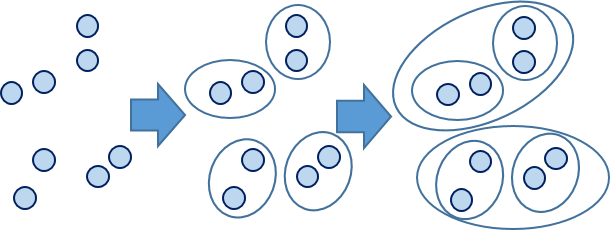
\includegraphics[width = 0.7\paperwidth] {multiscale_structure.png}
\]
}
\frame{\frametitle{Plan}
\begin{itemize}
\item There are relatively intuitive ways of clustering: We could connect points within $k$ of each other and then scale $k$.
\item But that's boring!
\end{itemize}
}
\section{Metric Spaces}


\frame{\frametitle{Definition}
\begin{itemize}
\item
A \textbf{metric space} $(X,d)$ is a set $X$ along with a function $d:X \times X \rightarrow \Rr^{\geq 0}$, such that, $\forall x,y,z \in X$:\\
\begin{itemize}
\item $d(x,y) \geq 0$, with equality iff $x = y$;
\item $d(x,y) = d(y,x)$; and
\item $d(x,y) + d(y,x) \geq d(x,z)$.
\end{itemize} 
If $X$ is finite then we say $(X,d)$ is a \textbf{finite metric space}.\\
\item
Useful example: Finite set of points in $\Rr^2$.
\end{itemize}
}

\frame{\frametitle{Data as a Metric Space}
\begin{itemize}
\item Data consists of a finite set of samples over $n$ variables
\item Very common idea: Represent data as points in $\Rr^n$. 
\item Note: $\Rr^n$ has far more structure than we need. We only care about distance.
\end{itemize}
}

\section{Weights}
\frame{\frametitle{Intuition behind Weighting}
\begin{itemize}
\item We want to count the number of clusters in a data set. So we'll assign a \textbf{weighting} to the points.
\item We want each cluster's weight to sum to close to 1
\item Points near many other points will have smaller values
\item Points which are separated will have larger values
\item Then, we'll sum the weights to get the \textbf{magnitude}, i.e. number of clusters, in the data set.
\end{itemize}
}
\frame{\frametitle{Weighting and Magnitude}
\begin{itemize}
\item
A \textbf{weighting} on a finite metric space $X$ is a set of weights $\omega_x$ in $\Rr$ such that, for all $x \in X$:
\[
\sum_{y \in X}e^{-d(x,y)}\omega_y = 1
\]
Weights may be negative, but it's easier to think of them as nonnegative.
\item Then the \textbf{magnitude} of $X$, denoted $|X|$, is defined by:
\[
|X| = \sum_{x \in X}\omega_x.
\]
\item May be various weightings, but magnitude is unique
\item Scale-dependent - see examples to come
\end{itemize}
}
\section{Examples}
\frame{\frametitle{Two Points}
Consider the space of two points separated by distance $d$:\\

                        \[
\begin{tikzpicture}[auto, node distance = 3cm, main node/.style={dot}]
\node[circle, draw, fill=black,
                        inner sep=0pt, minimum width=4pt](1) at (0,0) {};
\node[circle, draw, fill=black,
                        inner sep=0pt, minimum width=4pt](2) at (4,0) {};

\draw (1) -- (2) node[midway, above] {\textit{d}};

\end{tikzpicture}\]
\begin{itemize}
\item If $d$ is small, we expect there to be one cluster, and if $d$ is large, 2 clusters.
\item In this case, the weight of each point is equal to 
\[\frac{1}{1+e^{-d}}\]
so the magnitude is
\[
\frac{2}{1+e^{-d}}.
\]
\end{itemize}
}
\frame{\frametitle{Two Points Plot}
The space's magnitude as we scale $d$:
}
\frame{\frametitle{Simple Examples}
Consider the space below:\\

                        \[
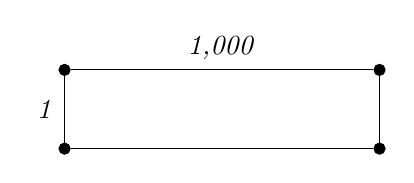
\begin{tikzpicture}[auto, node distance = 3cm, main node/.style={dot}]
\node[circle, draw, fill=black,
                        inner sep=0pt, minimum width=4pt](1) at (0,0) {};
\node[circle, draw, fill=black,
                        inner sep=0pt, minimum width=4pt](2) at (4,0) {};
\node[circle, draw, fill=black,
                        inner sep=0pt, minimum width=4pt](3) at (0,-1) {};
\node[circle, draw, fill=black,
                        inner sep=0pt, minimum width=4pt](4) at (4,-1) {};
\draw (1) -- (2) node[midway, above] {\textit{1,000}};
\draw (1) -- (3)node[midway, left] {\textit{1}};
\draw (2) -- (4);
\draw (3) -- (4);
\end{tikzpicture}\]
\begin{itemize}
\item If $d$ is small, we expect there to be one cluster, and if $d$ is large, 2 clusters.
\item In this case, the weight of each point is equal to 
\[\frac{1}{1+e^{-d}}.\]
\end{itemize}
}

\section{}


\frame{\frametitle{}
\begin{center} {\huge Thank you!}\end{center}
}

\end{document}

